\documentclass{article}
\usepackage[usenames]{color} %used for font color
\usepackage{amssymb} %maths
\usepackage{amsmath} %maths
\usepackage[utf8]{inputenc} %useful to type directly diacritic characters
%\usepackage[linesnumbered,ruled,vlined]{algorithm2e}
\addtolength{\topmargin}{-.975in}
%\pagenumbering{gobble}
\usepackage{url}
%\usepackage{hyperref}
\usepackage{float}
\usepackage{pgfplots}
\usepackage{tikz}
\usepackage{graphicx}
\usepackage[french]{babel}




\title{Second Rapport INF6404A : Présentation du Middleware}
\author{
	Alexandre Mao\\
	David Johannès \\
	Philippe Troclet \\
	Fabien Berquez \\
	D\'{e}partement G\'{e}nie Informatique et G\'{e}nie Logiciel \\
	\'{E}cole Polytechnique de Montr\'{e}al, Qu\'{e}bec, Canada \\
	\texttt{alexandre.mao@polymtl.ca}\\
	\texttt{david.johannes@polymtl.ca}\\
	\texttt{philippe.troclet@polymtl.ca}   \\
	\texttt{fabien.berquez@polymtl.ca}   \\
}
\date{19 mai 2016}

\usepackage{natbib}
\usepackage{graphicx}

\begin{document}

\maketitle

\section{Introduction}
Le monde d’IoT représente par définition un système “intégré”, où les différents objets interagissent entre eux, sont
inter-connectés, à travers l’échange d’informations et de commandes (requête, demande). Ces objets ont une forte probabilité d’être hétérogènes en termes de niveau de sécurité, de privacité minimal garanti, de technologie, de protocole de communication, et de politique d’exécution. Le challenge est ainsi davantage lié au besoin d’avoir une structure horizontale capable de gérer les spécifications de sécurité et de privacité de manière unique et homogène. Ces spécifications auront besoin en effet d’être instanciées sur des “entités” et auront potentiellement des interfaces d’implémentation, de spécification et de communication différentes.
\\

Les caractéristiques de IoT comprennent donc un réseau à très grande échelle des objets, une grande hétérogénéité au niveau des dispositifs et du réseau, et un grand nombre d'événements générés spontanément par ces objets. Malheureusement, toutes ces caractéristiques feront du développement des diverses applications et des services une tâche très difficile. En général, le middleware peut faciliter un processus de développement en intégrant des dispositifs informatiques et de communication hétérogènes, et en soutenant l'interopérabilité au sein des diverses applications et services.

En effet, un middleware fait abstraction de la complexité du système ou du matériel, permettant au développeur d'applications de concentrer tous ses efforts sur la tâche à résoudre, sans la distraction des préoccupations orthogonales au niveau du système ou du matériel. Ces complexités peuvent être liées à des préoccupations de communication ou au calcul plus généralement. Un middleware fournit une couche logicielle entre les applications, le système d'exploitation, les couches de communication réseau et les différents dispositifs du système, ce qui facilite et coordonne certains aspects du traitement coopératif. Du point de vue informatique, un middleware fournit une couche entre les logiciels d'application et des logiciels système. Dans l'IoT, l’hétérogénéité des dispositifs implique très souvent une hétérogénéité considérable dans les technologies de communication utilisées, ainsi que dans les technologies au niveau du système, c’est pourquoi un middleware devrait supporter ces deux types d’hétérogénéité. Nous avons donc besoin d’un middleware qui respecte des caractéristiques, que nous décrirons par des modules. Ces modules seront divisés en trois groupes : les modules fonctionnels, liés aux services et aux fonctions que notre middleware doit fournir ; les modules non-fonctionnels, liés à la Quality of Service (QoS), aux performances et aux différentes exigences que notre middleware devra prendre en compte; et les modules architecturaux, liés à l’architecture de notre middleware.
\\
\begin{figure}[h!]
	\hspace*{-1cm}
	\centering
	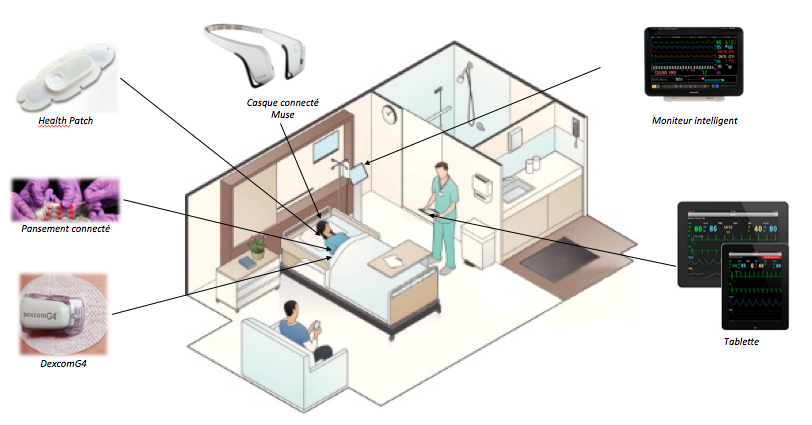
\includegraphics[width=1.1\textwidth]{Figure1.png}
	\caption{Couches Dispositifs, et Protocoles de Réseau et de Communication de notre Système}
	\label{fig:couches}
\end{figure}

Rappelons que notre sujet consiste à établir un système IoT dans le domaine Smart Health, et plus précisément dans les services de
soins intensifs des hôpitaux, afin de résoudre le problèmes de congestion et de surveillance en continu dans ces services. La Figure
\ref{fig:couches} nous permet de visualiser les choix de dispositifs et de protocoles de communication et de réseau que nous avons établis
dans le rapport précédent. Avant de commencer à décrire les différents modules dont nous aurons besoin dans notre middleware, ce que nous feront dans les section 2, 3, et 4, il est important de préciser le choix que nous avons fait concernant l’architecture générale de notre middleware. En effet, nous avons décidé de diviser notre middleware en deux couches différentes, la première étant liée au moniteur qui centralise toutes les informations des divers dispositifs présents dans la chambre du patient, et qui donc va gérer l’hétérogénéité entre les dispositifs présents dans l’environnement du patient. La seconde couche middleware est liée au Gateway de notre système, qui s’occupe de centraliser les informations de tous les moniteurs (le problème d’hétérogénéité se pose moins ici), et qui va faire le lien entre la couche de stockage et celle de liaison à la couche physique. Cette seconde couche va être celle qui permettra d’identifier les différents groupements de dispositifs à travers la connaissance des différents moniteurs intelligents.

La Figure \ref{fig:vueglobale} nous permet de visualiser la structure de notre système en considérant seulement les couches dispositifs, réseaux et communication, middleware, et architecture. Ainsi, dans les trois prochaines sections, notre tâche ne sera pas seulement de décrire les différents modules dont nous avons besoin dans notre middleware, mais aussi de décrire dans quelle(s) couche(s) middleware nous en avons besoin (possiblement les deux).

\begin{figure}[h!]
	\hspace*{-2.5cm}
	\centering
	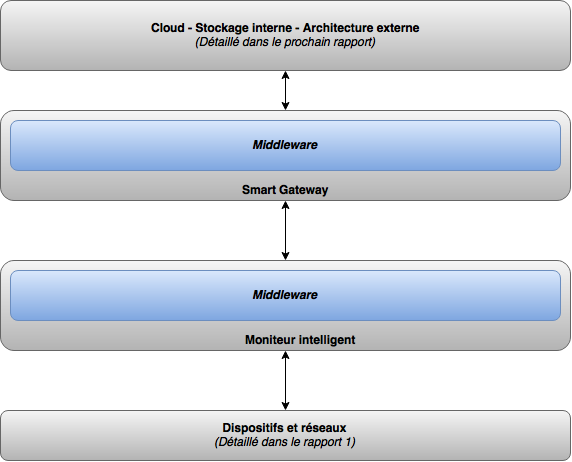
\includegraphics[width=1.4\textwidth]{Figure2.png}
	\caption{Vue Globale de notre Middleware au sein de notre Système}
	\label{fig:vueglobale}
\end{figure}


\section{Les Exigences du Middleware}
Figure 3 pour résumer les exigences dans notre Middleware.
\subsection{Les Éxigences Fonctionnelles}
Les exigences fonctionnelles du Middleware correspondent aux services et aux fonctions qu’un middleware doit fournir, et sont donc représentées par la découverte des ressources, et toute forme de gestion (gestion des données, des ressources, des événements et du code).
\\

Tout d'abord, une des exigences les plus significatives du Middleware est la \textbf{\textit{découverte des ressources}}. Les ressources IoT comprennent les dispositifs hétérogènes de matériel (par exemple les étiquettes RFID, les capteurs, et les smartphones), la puissance et la mémoire des dispositifs, analogues à des dispositifs de conversion numérique (A/D), le module de communication disponible sur ces appareils, les informations au niveau de l'infrastructure ou du réseau (par exemple la topologie du réseau et des protocoles), et les services fournis par ces dispositifs. Les hypothèses relatives aux connaissances globales et déterministes de la disponibilité de ces ressources ne sont pas valides, car l'infrastructure et l'environnement de l'IoT est dynamique (les dispositifs, et leur nombre seront différents en fonction du patient qui est reçu). Ainsi, l'intervention humaine pour la découverte de ressources est infaisable et, par conséquent, une condition importante pour la découverte de ressources est qu'elle doit être automatisée. Par ailleurs, lorsqu'il n'y a pas de réseau d'infrastructure, chaque appareil doit annoncer sa présence et les ressources qu'il offre.

\textbf{\textit{La gestion des ressources}} est une exigence importante qui entre en jeu naturellement après la découverte des ressources du Middleware, car elle se réfère à la qualité de service (QoS ou Quality of Service). En effet, une QoS acceptable est attendue pour toutes les applications, et dans un environnement où les ressources ayant un impact sur la qualité de service sont limitées, comme l'IoT, il est important que les applications soient fournies avec un service qui gère ces ressources. Cela signifie que l'utilisation des ressources doit être surveillée, que les ressources allouées ou provisionnées le soient de manière équitable, et que les conflits de ressources soient résolus.

\textbf{\textit{La gestion des données}} est également une caractéristique primordiale au sein du Middleware. Dans l'IoT, les données se réfèrent principalement aux données détectées ou toute autre information d'infrastructure de réseau d'intérêt pour les applications. Ainsi, un middleware IoT doit fournir des services de gestion des données pour les applications, y compris l'acquisition de données, le traitement des données (incluant le prétraitement des données), et le stockage de données. C'est une exigence importante à respecter dans notre cas car il faut récupérer les données des différents dispositifs, puis les traiter, et les interpréter, ce que nous décrirons par la suite à travers certains modules de notre Middleware.

Comme nous avons un système qui dépend des événements, la gestion de ceux-ci est aussi une exigence à considérer dans notre solution IoT. Il y a en effet potentiellement un grand nombre d'événements générés dans les applications IoT, qui devraient être gérés comme une partie intégrante d'un middleware IoT.  \textbf{\textit{La gestion des événements}} transforme les événements observés simples en des événements significatifs. C'est donc une exigence importante dans notre cas pour gérer les alertes, que ce soit au niveau des pannes des dispositifs, mais aussi au niveau des urgences (qui nécessitent l’intervention de personnel soignant).

Enfin, en temps qu'exigence fonctionnelle, il est nécessaire d'avoir une certaine \textbf{\textit{gestion du code}}, car le déploiement du code dans un environnement IoT est difficile, et doit être directement pris en charge par le Middleware. En particulier, les services d'allocation de code et de migration de code sont nécessaires, et il est possible que les technologies en terme de dispositifs et de protocoles de communication et de réseau évoluent.
\subsection{Les Exigences Non-Fonctionnelles}
Les middlewares ont un rôle important dans tout système d’IoT, et ce sont eux qui vont faire la transition entre les objets connectés et les couches supérieures, notamment celles de stockage. C’est pourquoi nous avons mis en évidence les différentes exigences non fonctionnelles du middleware suivantes par rapport à notre système.
\\

\textbf{\textit{L'évolutivité}} correspond au fait qu'un middleware d’un système de l’IoT doit pouvoir évoluer pour pouvoir répondre à l’expansion du réseau et à l’ajout d’applications et de services. Dans notre cas, l’évolutivité du middleware doit pouvoir prendre en compte l’ajout d’éventuels capteurs, et différents objets connectés. Il doit par ailleurs laisser la possibilité de fournir des services supplé\-mentaires ainsi que des applications diverses en fonction des besoins.

Il faut permettre au middleware de respecter l'\textbf{\textit{exigence du temps réel}}. En effet, certains middlewares doivent pouvoir fournir des informations ou des services en temps réel lorsque la correction d'une opération qu’il prend en charge dépend non seulement de la correction logique, mais aussi du temps pendant lequel cette opération est réalisée. De nombreuses applications en temps réel vont utiliser les données fournies. L’envoi et la réception à temps des informations ou des services dans ces applications sont alors essentiels. Certains capteurs que nous avons proposés ont pour but de surveiller des données vitales sur le patient, par conséquent ces informations doivent pouvoir être consultées en temps réel car des délais de transmission peuvent avoir des conséquences graves voire mortelles sur un patient.

\textbf{\textit{La fiabilité}} d'un middleware est une exigence essentielle. Un middleware doit rester opérationnel pendant toute la durée d'une mission, même en présence de pannes. La fiabilité du middleware aide en dernier recours la réalisation de la fiabilité au niveau du système. Chaque composant ou service dans un middleware doit être fiable pour atteindre la fiabilité globale, ce qui inclut celles de la communication, des données, des technologies et des dispositifs de toutes les couches. Les signes vitaux qui sont surveillés imposent au middleware d’être capable de transmettre les données de façon fiable sans corruption de celles-ci, et cela toujours à cause des données qui sont surveillées.

Il y a la nécessité également d'introduire \textbf{\textit{la disponibilité}} au sein de notre middleware. En effet, même s'il y a une défaillance quelque part dans le système, le temps de récupération et la fréquence de défaillance de celui-ci doivent être suffisamment petits pour obtenir la disponibilité souhaitée. Les exigences en matière de fiabilité et de disponibilité doivent travailler ensemble pour assurer la plus haute tolérance aux pannes nécessaire depuis une application. Le middleware doit pouvoir être capable de détecter si l’un de nos capteurs est en panne, et pour cela, il va faire des requêtes à intervalles réguliers des signes vitaux et en cas d’absence de réponse pendant un temps prédéfini, une alerte sera envoyée au personnel médical pour vérifier l’origine de l’erreur. Dans le domaine de la santé, où la vie des patients est en jeu, nous ne pouvons pas nous permettre de laisser le patient sans surveillance médicale.

\textbf{\textit{La sécurité}} et \textbf{\textit{la privacité}} sont des exigences à ne pas oublier dans un tel système qu'est le nôtre. La sécurité doit être prise en compte dans tous les blocs fonctionnels et non fonctionnels. Nous avons différentes couches de sécurité dans les parties de notre architecture. Tout d’abord au niveau de l’identification des appareils connectés, nous proposons un système d’identification des appareils auprès du moniteur intelligent, ce qui évitera la connexion de capteurs non souhaités, et nous pourrons aussi dans l’autre sens connecter un capteur qu’à un seul moniteur. Au niveau de nos moniteurs intelligents, il y aura la mise en place d’un système de chiffrement des données pour l’envoi à la couche supérieure pour préserver la confidentialité des données envoyées du patient.

\textbf{\textit{La facilité de déploiement}} est également une exigence que nous visons au sein de notre middleware, car le déploiement ne devrait pas exiger des connaissances spécialisées, et les procédures d'installation et de configuration compliquées devraient être évitées. Dans notre cas l’ajout de capteur se fera à travers une interface simple sur le moniteur intelligent qui identifiera cet appareil au réseau mère. Et ainsi, l’ajout de nouveaux dispositifs se fera de manière aisée.
\subsection{Les Exigences Architecturales}
Les exigences de Middleware abordées ici sont universelles, car applicables à n'importe quel Middleware, et concerne les exigences architecturales des Middlewares.
\\

L'architecture de notre Middleware doit tout d'abord présenter une abstraction de la programmation, c'est-à-dire fournir une API (Interface de Programmation Applicative) pour les développeurs d'application. C'est une exigence fonctionnelle importante pour tout middleware. Pour le développeur de l'application ou du service, des interfaces de programmation de haut niveau ont besoin d'isoler le développement des applications ou des services provenant des opérations prévues par les infrastructures IoT hétérogènes et sous-jacentes. Le niveau d'abstraction, le paradigme de programmation, et le type d'interface doivent tous être pris en considération lors de la définition d'une API.

L'architecture de notre Middleware doit aussi être interopérable. Un middleware devrait en effet fonctionner avec des appareils, des technologies, ou des applications hétérogènes sans effort supplémentaire de la part du développeur de l'application ou du service. Les composants hétérogènes doivent être en mesure d'échanger des données et des services. L'interopérabilité dans un middleware peut être observée à partir du réseau, des perspectives sémantiques et syntaxiques, et chacun doit être pris en charge dans un IoT.

Notre Middleware doit être basé sur les services. Une architecture de middleware devrait être basée sur les services afin d’offrir une grande flexibilité lorsque les fonctions nouvelles et avancées doivent être ajoutées au middleware IoT. Un middleware basé sur les services fournit des abstractions pour le matériel sous-jacent complexe à travers un ensemble de services (par exemple la gestion des données, la fiabilité, la sécurité) nécessaires pour les applications.

L'architecture de notre Middleware doit être adaptable. En effet, un middleware doit être adapté afin qu'il puisse évoluer pour s'accorder à des changements dans son environnement. Dans l'IoT, le réseau et son environnement sont susceptibles de changer fréquemment. En outre, les demandes ou le contexte au niveau de l'application sont également susceptibles de changer fréquemment. Afin d'assurer la satisfaction des utilisateurs et l'efficacité de l'IoT, un middleware doit s’adapter dynamiquement ou s'ajuster à toutes ces variations.

Un middleware doit être context-aware (attentif au contexte), c'est-à-dire conscient du contexte des utilisateurs, des dispositifs, et de l’environnement et utiliser ce contexte pour des offres de services efficaces et essentiels pour les utilisateurs.

Notre middleware doit bien évidemment présenter une certaine autonomie. Les appareils, les technologies, ou les applications sont des participants actifs dans les processus de l'IoT et ils devraient pouvoir interagir et communiquer entre eux sans intervention humaine directe. L'utilisation de l'intelligence, y compris des agents autonomes, de l’intelligence embarquée, et des approches prédictives et proactives dans le middleware peut satisfaire cette exigence.

Enfin, comme nous le montre en partie la Figue 2, notre Middleware doit être distribué. En effet, les applications, les dispositifs, et les utilisateurs sont susceptibles d'être distribués géographiquement, et donc une mise en oeuvre d’une vue ou d’un middleware centralisé ne sera pas suffisant pour supporter de nombreux services ou applications distribuées. Une implémentation d'un middleware doit prendre en charge les fonctions qui sont distribuées à travers l'infrastructure physique de l'IoT.

\section{Intergiciel - Middleware}
\subsection{Middleware niveau moniteur}
Dans cette partie, nous allons nous intéresser au middleware présent au niveau du moniteur, comme illustré à la Figure \ref{4}. Afin de contextualiser, nous allons rappeler les fonctionnalités principales de ce dernier. Tout d'abord, il a un rôle d'agrégateur \cite{li2015iot}, il doit donc rassembler les données issues de différents capteurs et les envoyer vers la passerelle intelligente via un unique message. 
\newline
\begin{figure}[h!]
	\hspace*{-3cm}
	\centering
	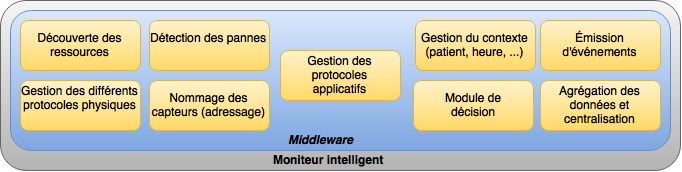
\includegraphics[width=1.5\textwidth]{Figure4.png}
	\caption{Middleware au niveau du Moniteur}
	\label{4}
\end{figure}

Ce requis impose de pouvoir comprendre différents protocoles, tant au niveau physique qu'applicatif, ainsi que différents formats. Il est en effet peu probable que tous les capteurs utilisent le même protocole pour la transmission de leurs données. Il est également nécessaire de permettre l'évolutivité au sein du système afin que de futurs capteurs plus performants, qui pourraient utiliser une nouvelle façon de communiquer, puissent être intégrés au système. Ceci sera géré par les modules de \textbf{\textit{gestion des différents protocoles physiques}} et \textbf{\textit{gestion des protocoles applicatifs}}.
\newline

De plus, afin d'optimiser le temps du personnel médical, le moniteur et donc le middleware va faciliter la découverte de capteurs ainsi que la récupération de leur contexte, ce qui sera rendu possible par le module de \textbf{\textit{découverte des ressources}}. Dans le TP1 nous avons évoqué la transmission de données depuis les capteurs. Pour que ces données aient une réelle signification, il faut que notre système soit conscient du type des données et des unités dans lesquelles ces données sont exprimées. Lorsqu’un capteur est rajouté au réseau des capteurs, il s’enregistre auprès du moniteur intelligent, il envoie ses propriétés, qui sont le type de données et les unités associées. Le moniteur peut ainsi stocker dans sa table de correspondance le protocole physique, le canal de communication, le type de données et l’unité associée, ainsi que le nom que le moniteur intelligent attribue au capteur qui vient de s’enregistrer. Ce nom est transmis au capteur qui peut alors le retenir. Se faisant, le moniteur est conscient, pour les données qu’il reçoit, de leur sémantique et des unités associées. Lors de l’agrégation des données et avant leur envoi à la Smart Gateway, le moniteur intelligent peut associer pour chaque type de données récupérées les unités associées dans un ou plusieurs paquets IPv4/IPv6 envoyés à la Smart Gateway. Ce processus est illustré par la Figure \ref{5}.
\newline
\begin{figure}[h!]
	\hspace*{-3cm}
	\centering
	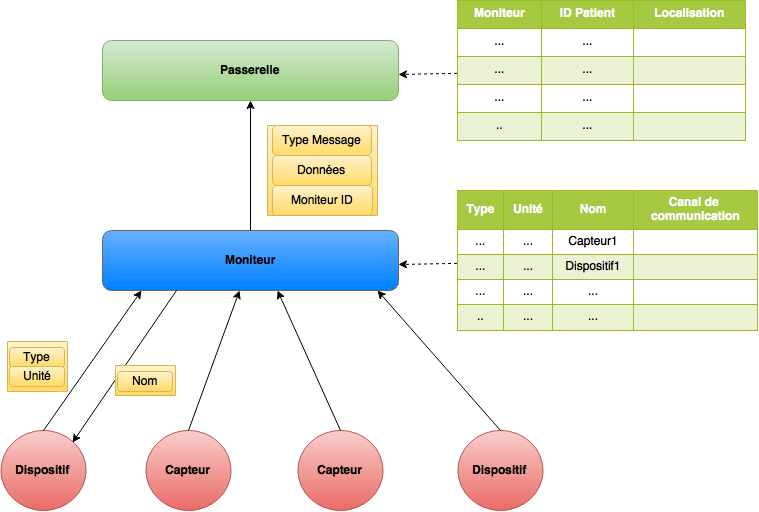
\includegraphics[width=1.5\textwidth]{Figure5.png}
	\caption{Découverte des Ressources et Gestion des Données}
	\label{5}
\end{figure}

Une fois les capteurs installés et découverts, le lien entre les données reçues, leurs unités et l'identité du patient devrait être fait automatiquement (ou presque), ce qu'assurera le module de \textbf{\textit{gestion du contexte}}. Cette étape intervient lorsque les données sont agrégées et préparées pour leur transmission par le module d'\textbf{\textit{agrégation des données}}.

Ces mêmes capteurs devraient être accessibles depuis l'extérieur. En effet, pour certaines données relevées rarement, il est possible qu'un médecin souhaite les rafraîchir plutôt que d'attendre la prochaine mise à jour. Il se peut également que le médecin, ou un outil automatique tel que le moniteur central, désire donner un ordre à un des objets intelligents. Pour cela, il faut que ces objets aient un nom, ou du moins soient adressables par un site d'identification unique. En particulier, un nom du type \textit{idPatient@typeDeCapteur} serait particulièrement pratique à utiliser. Le module de \textbf{\textit{nommage des capteurs}} répondra à ce problème. Il peut être nécessaire, dans le cas de décisions automatisées (par exemple la régulation d'un débit de perfusion, ...), que le middleware comprenne un \textbf{\textit{module de décision}} pour lequel des règles pourraient être définies afin qu'il actionne des objets connectés présents dans l'environnement du patient.
\newline

Enfin, il est impératif, dans la mesure du possible, de sécuriser les communications au sein du système. Cela passe par un
contrôle d'accès au niveau du moniteur avec un mécanisme d'authentification. Mais aussi par une \textbf{\textit{détection des pannes}}, qui sera géré par un module propre. En effet, il
est souhaitable, de part l'importance des données fournies par ces capteurs, qu'ils soient remplacés dès le premier indice
de dysfonctionnement. De manière générale, il est important de garantir une bonne disponibilité ainsi qu'une certaine fiabilité.
\newline

Ces considérations sur la détection de pannes entrainent également la nécessité de disposer d'un module d'\textbf{\textit{émission d'évènements}} afin que le middleware du moniteur intelligent puisse avertir immédiatement la Smart Gateway d'un dysfonctionnement d'un capteur, ou d'une valeur anormale par rapport au profil du patient (par exemple une crise cardiaque).
\newline

\begin{table}[h!]
	\hspace*{-4.5cm}
    \centering
    \begin{tabular}{|l|c|c|c|c|c|c|c|c|c|c|}
        \hline
        Modules & \begin{tabular}[c]{@{}l@{}} Découverte \\ ressources \end{tabular} & Scalabilité & \begin{tabular}[c]{@{}l@{}} Interopéra- \\ -bilité \end{tabular} & \begin{tabular}[c]{@{}l@{}} Adapta- \\ -bilité \end{tabular} & Fiabilité & \begin{tabular}[c]{@{}l@{}} Disponi- \\ -bilité \end{tabular} &  \begin{tabular}[c]{@{}l@{}} Temps \\
        réel \end{tabular} & \begin{tabular}[c]{@{}l@{}} Basé \\ sur les \\ services \end{tabular} &  \begin{tabular}[c]{@{}l@{}} Context \\ aware \end{tabular} & Autonome\\
        \hline
        \hline
        \begin{tabular}[c]{@{}l@{}}Découverte \\ des \\ ressources \end{tabular} & \checkmark & \checkmark & & \checkmark & & & & &&\\
        \hline
        \begin{tabular}[c]{@{}l@{}}Détection \\ panne \end{tabular} & & & & & \checkmark & \checkmark & \checkmark &  \checkmark && \\
        \hline
        Décision & & \checkmark & & \checkmark & \checkmark & \checkmark & & & & \checkmark \\
        \hline
        \begin{tabular}[c]{@{}l@{}}Gestion \\ du \\ contexte \end{tabular} & & & && & &&& & \checkmark \\
        \hline
        \begin{tabular}[c]{@{}l@{}}Émission \\ d'événements \end{tabular} & & & \checkmark & \checkmark & & \checkmark & & & \checkmark & \\
        \hline
        \begin{tabular}[c]{@{}l@{}}Gestion des \\ différents \\ protocoles \\ physiques \end{tabular} & & \checkmark & && & & & & & \\
        \hline
        \begin{tabular}[c]{@{}l@{}}Nommage \\ des capteurs \end{tabular} & & \checkmark & \checkmark & \checkmark && & & & & \\
        \hline
        \begin{tabular}[c]{@{}l@{}} Agrégation \\ de données et \\ centralisation  \end{tabular} & & \checkmark & \checkmark & \checkmark & & & & & & \\
        \hline
        \begin{tabular}[c]{@{}l@{}} Gestion des \\ différents \\ protocoles \\ applicatifs \end{tabular} & & \checkmark & \checkmark & \checkmark & & & & & &\\
        \hline
    \end{tabular}
    \caption{Utilisation des services du middleware par les différents modules}
\end{table}

\begin{table}[h!]
	\hspace*{-4cm}
    \centering
    \begin{tabular}{|l|c|c|c|c|}
        \hline
        Modules & Gestion ressources & Gestion données & Gestion événements & Gestion du code \\
        \hline
        \hline
        Découverte des ressources & \checkmark & & & \\
        \hline
        Détection panne & \checkmark & & & \\
        \hline
        Décision & & & &\\
        \hline
        Gestion du contexte & & \checkmark & \checkmark & \\
        \hline
        Émission d'événements & & \checkmark & \checkmark & \\
        \hline
        Gestion des différents protocoles physiques & & & & \checkmark \\
        \hline
        Nommage des capteurs & \checkmark & & & \\
        \hline
        Agrégation de données et centralisation & & \checkmark & & \\
        \hline
        Gestion des différents protocoles applicatifs & & & & \checkmark \\
        \hline
    \end{tabular}
    \caption{Utilisation des services de gestion du middleware par les différents modules}
\end{table}

Les tableaux 1 et 2 présentent les modules sur la première colonne avec les exigences du middleware sur la première ligne.
\newline

Par ailleurs, il serait nécessaire de présenter une API simple d'utilisation au niveau du middleware afin de faciliter la programmation de nouvelles fonctionnalités et l'utilisation des services offerts par des applications extérieures.
	
\subsection{Middleware niveau gateway}
La smart Gateway présente un rôle central dans notre architecture, c’est elle qui va faire l’intermédiaire entre les parties plus bas niveau comprenant les dispositifs et le middleware s’occupant de gérer ces dispositifs, et la partie supérieure qui correspond au reste de l’application avec le stockage des données, et les différentes applications. La Figure \ref{gateway} illustre le middleware que nous avons adopté au niveau du Gateway.
\newline
\begin{figure}[h!]
	\hspace*{-3cm}
	\centering
	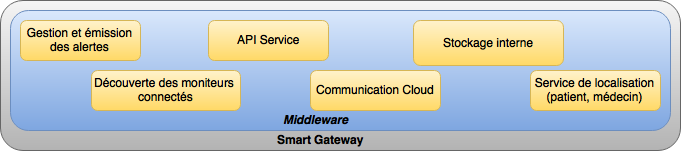
\includegraphics[width=1.5\textwidth]{Figure6.png}
	\caption{Middleware au niveau du Gateway}
	\label{gateway}
\end{figure}

Dans notre cas, elle va avoir différents modules pour répondre aux exigences du système. Elle aura un rôle primordial dans la transmission en temps réel des alertes depuis les couches inférieures, pour cela, un module autonome de \textbf{\textit{gestion et d’émission des alertes}} sera présent pour pouvoir recevoir et réémettre aux bons destinataires ou aux bonnes applications les alertes. Ce module pourra être couplé avec un module de \textbf{\textit{localisation du personnel médical et du patient}}, pour que l’alerte soit déclenchée dans la zone proche du patient et qu’elle atteigne le personnel médical compétent pour agir sur cette urgence tout en leur signalant la localisation de l’urgence. Ce module aura besoin d’être fiable et disponible dans la gestion des événements qu’il reçoit car ceux-ci peuvent être des alertes vitales sur des patients.

L’identification des patients, et leur localisation dans l’hôpital étant une nécessité, la présence d’un module permettant d’ajouter au réseau les nouveaux moniteurs connectés est indispensable. Dans l’architecture que nous proposons, nous avons un module dédié à la recherche des appareils, qui dans ce middleware sera la \textbf{\textit{recherche des moniteurs intelligents}}. Les appareils de plus bas niveau vont se déclarer à ceux de plus haut niveau pour que ces derniers puissent les identifier de manière unique et leur associer les bonnes informations. Dans notre cas par exemple, lors de l’installation d’un nouveau patient, le moniteur va rechercher ou recevoir l’identifiant du patient, et une fois connectée au réseau, il se déclarera auprès de la passerelle intelligente pour que celle-ci puisse mettre en mémoire la correspondance entre le moniteur et le patient. Une fois l’élément entré dans la table de correspondance de la passerelle intelligente, toutes les informations fournies par le moniteur pourront être transmises de manière cohérente auprès de la passerelle qui fera la redirection pour le stockage ou l’interprétation des données. Et la passerelle intelligente, informera ensuite le serveur IoT et les éventuelles autres passerelles de la présence de ce nouvel élément. La méthode de recherche des dispositifs que nous proposons permettra une évolutivité et une adaptabilité aisées du système.\cite{li2015iot}

Une fois que la passerelle intelligente a pris connaissance des moniteurs connectés dans sa zone de couverture, elle va avoir pour rôle de transmettre les différentes informations de ces moniteurs pour leur stockage. Elle va donc s’occuper de gérer les données reçues avec l’aide d’un \textbf{\textit{module de communication Cloud}}, qui s’occupera de faire l’intermédiaire entre les couches de stockage et les couches supérieures. Pour cela elle doit être capable de communiquer avec les moyens de stockage que nous proposons sous forme de Cloud. Ce module s’occupera donc de la gestion des données, et sera donc couplé avec \textbf{\textit{un module de stockage interne}}, qui servira de table de correspondances entre les différents moniteurs intelligents et le patient auquel il réfère. Le module de stockage interne servira à avoir le contexte des données qui sont fournies.

Comme nous avons pu le voir jusqu’à maintenant, le middleware présent au niveau du Smart Gateway a un rôle primordial dans le traitement et la redirection des informations. Il doit être capable de faire ces différentes tâches en prenant en compte la sécurité des données qui transitent. La Smart Gateway va avoir un module d’authentification et de contrôle d’accès pour restreindre l’accès à ces données et éviter le vol de données privées sur les patients. Les applications dans le domaine de la santé recueillent des informations confidentielles sur les patients, et l’exposition de ces informations peut avoir des conséquences sur la vie privée et professionnelle de ces personnes. C’est pourquoi nous incorporons différents modules de sécurité dans les différentes couches de notre système. La Smart Gateway va ainsi posséder un module de chiffrement des communications pour garder la confidentialité des données qui sont transmises. Le couplage de ce module avec un module d’authentification et de contrôle d’accès va nous permettre d’avoir des mesures de sécurité quant aux informations des patients.

Enfin pour l’évolutivité du système proposé ainsi que l’ajout de différentes fonctionnalités, nous proposons un module \textbf{\textit{API service}} qui contiendra les différentes API nécessaires à l'utilisation des services offerts par le middleware depuis les autres plateformes. Nous aurons donc une abstraction du code qui permettra une utilisation aisée des services disponibles.

Le middleware sera de plus construit sur un système d'extensions (plug-in) afin de rendre facile l’ajout de fonctionnalités à la Smart Gateway, comme par exemple l’introduction de nouveaux services, types de capteurs. Ceci améliorera l'évolutivité et l'adaptabilité de notre système.

\subsection{La sécurité dans le middleware}
La vie privée et la sécurité sont des préoccupations majeures dans les systèmes IoT, et en particulier dans notre système centré autour de la santé. En effet, les données, en cas de fuite ou de corruption par un agent extérieur, sont susceptibles d'avoir des conséquences graves sur la vie du patient. Notre middleware doit donc prendre en compte cette problématique et répondre à ces défis. Comme la sécurité est un problème transverse, n'étant pas limité à l'un des maillons du système, nous avons choisi de l'évoquer dans cette partie séparée. \\Après l'étude des risques potentiels, nous avons défini les modules suivants pour offrir des services et des garanties concernant la sécurité :\\
\begin{itemize}
\item \textbf{\textit{Authentification :}} Il s'agit d'un module destiné à s'assurer et attester de l'identité d'un service, d'une application ou d'un utilisateur faisant une requête ou donnant un ordre à notre système, et particulièrement à notre middleware. L'objectif derrière ces considérations est de protéger le reste du système de requêtes provenant d'agents non-identifiés, tout en pouvant garantir l'origine des ordres, c'est à dire s'assurer qu'il n'est pas possible, pour une personne ou un service ayant fait une requête ou ayant transmis un ordre, de répudier l'avoir fait. Ceci est nécessaire à la fois pour la sécurité, mais aussi parfois pour des raisons de législation et de responsabilité devant la loi.
\item \textbf{\textit{Contrôle d'accès :}} Ce module, qui s'appuie tout d'abord sur le module d'\textit{authentification} intervient à l'étape suivante. Une fois le requérant identifié, il convient de s'assurer qu'il a le droit d'accéder, de visionner, de modifier ou de supprimer les données visées, qu'elles soient dans le Cloud ou dans le stockage local mis en place dans notre architecture. Parallèlement, ce module s'assure également qu'un ordre passé ne soit transmis que si l'utilisateur ou l'application demandeuse est autorisée à effectuer cette action. Ce module répond aux considérations à la fois de sécurité, mais aussi de privacité, en s'assurant que les données ne soit transmises qu'à des personnes ou des applications identifiées, autorisées et légitimes.
\item \textbf{\textit{Chiffrement des communications :}} Ce module a pour rôle de chiffrer les communications en utilisant les techniques de chiffrage appropriés afin de s'assurer qu'en cas de détournement des paquets, ou d'attaques de type Man In The Middle, les données sensibles comme le profil des patients, leur historique, leur dossier, les éléments venant de la base de données interne, ou du Cloud ou encore les informations de localisation des médecins ou des patients ne puissent être utilisés ou même consultés. Ce module agit pleinement pour favoriser la sécurité, mais plus encore la privacité. Il s'agit d'éviter ici les fuites de données personnelles, l'un des risques majeurs de l'IoT, renforcé par le caractère sensible des données transitant.
\item \textbf{\textit{Sécurité et intégrité des communications :}} Ce module est conçu pour s'assurer de la sécurité des communications, particulièrement celles orientées vers et depuis l'extérieur (par exemple le Cloud), mais aussi en interne entre les moniteurs et la Smart Gateway, ainsi que de l'intégrité des données reçues. En effet, une fois les données des capteurs agrégées (notamment avec le contexte) sur le moniteur, celles ci sont transmises à la Smart Gateway qui doit s'assurer de leur intégrité afin de ne pas enregistrer de fausses entrées. De même, certaines alertes étant générées par les moniteurs intelligents et transmises à la Smart Gateway pour leur transmission finale vers l'équipe médicale, il est important qu'aucun renseignement ne soit perdu au cours de ces transmissions. Ce module se concentre donc sur la sécurité, plus que la privacité des communications, car celle ci est renforcée par le module de chiffrement.\\
\end{itemize}
Ainsi, nous avons conçu cette partie transverse du middleware afin de s'assurer d'une sécurité et d'une protection de la vie privée maximale dans la limite des possibilités techniques. Les problématiques liées à la Qualité de Service (QoS) sont également pris en compte par la vérification de l'intégrité, donc de la fiabilité des données transmises, afin d'éviter des situations potentiellement risquées.
\subsection{Récapitulatif}
Figure 7.

\begin{figure}[h!]
	\hspace*{-1cm}
	\centering
	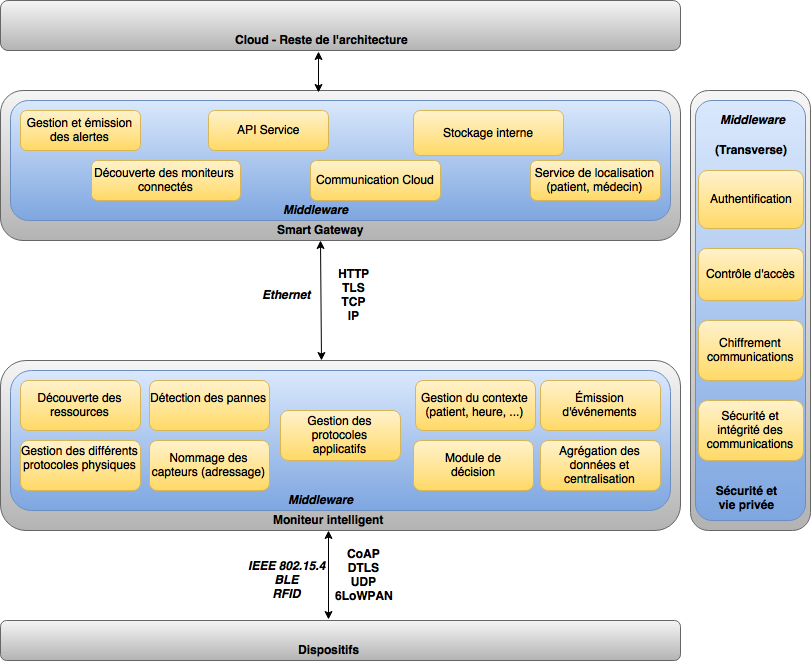
\includegraphics[width=1.1\textwidth]{Figure8.png}
	\caption{Le Middleware de notre Système et ses Modules}
	\label{fig:balance}
\end{figure}

\begin{table}[h!]
	\hspace*{-3cm}
	\centering
	\begin{tabular}{|l|c|c|c|c|c|}
		\hline
		\textbf{Modules}                                     & \textbf{\begin{tabular}[c]{@{}l@{}}Découverte \\ des \\ ressources\end{tabular}} & \textbf{\begin{tabular}[c]{@{}l@{}}Gestion \\ des \\ ressources\end{tabular}} & \textbf{\begin{tabular}[c]{@{}l@{}}Gestion \\ des \\ données\end{tabular}} & \textbf{\begin{tabular}[c]{@{}l@{}}Gestion \\ des \\ événements\end{tabular}} & \textbf{\begin{tabular}[c]{@{}l@{}}Gestion \\ du \\ code\end{tabular}} \\ \hline
		\hline
		\textit{Gestion et émission des alertes}             &                                                                                  &                                                                               &                                                                            & \checkmark                                                                    &                                                                        \\ \hline
		\textit{Communication Cloud}                         &                                                                                  &                                                                               & \checkmark                                                                 &                                                                               &                                                                        \\ \hline
		\textit{Service de localisation (patient, médecin)}  &                                                                                  & \checkmark                                                                    &                                                                            &                                                                               &                                                                        \\ \hline
		\textit{Découverte des moniteurs connectés}          & \checkmark                                                                       &                                                                               &                                                                            &                                                                               &                                                                        \\ \hline
		\textit{Stockage interne}                            &                                                                                  &                                                                               & \checkmark                                                                 &                                                                               &                                                                        \\ \hline
		\textit{API service}                                 &                                                                                  &                                                                               &                                                                            &                                                                               &                                                                        \\ \hline
		\hline                                                                              
		\textit{Découverte des ressources}                   & \checkmark                                                                       &                                                                               &                                                                            &                                                                               &                                                                        \\ \hline
		\textit{Détection des pannes}                        &                                                                                  & \checkmark                                                                    &                                                                            &                                                                               &                                                                        \\ \hline
		\textit{Décision}                                    &                                                                                  &                                                                               &                                                                            &                                                                               &                                                                        \\ \hline
		\textit{Gestion du contexte}                         &                                                                                  &                                                                               & \checkmark                                                                 & \checkmark                                                                    &                                                                        \\ \hline
		\textit{Emission d'événements}                       &                                                                                  &                                                                               & \checkmark                                                                 & \checkmark                                                                    &                                                                        \\ \hline
		\textit{Gestion des différents protocoles physiques} &                                                                                  &                                                                               &                                                                            &                                                                               & \checkmark                                                             \\ \hline
		\textit{Nommage des capteurs}                        &                                                                                  & \checkmark                                                                    &                                                                            &                                                                               &                                                                        \\ \hline
		\textit{Agrégation des données et centralisation}    &                                                                                  &                                                                               & \checkmark                                                                 &                                                                               &                                                                        \\ \hline
		\textit{Gestion des protocoles applicatifs}          &                                                                                  &                                                                               &                                                                            &                                                                               & \checkmark                                                             \\ \hline
	\end{tabular}
	\caption{Modules de notre Middleware et Exigences Fonctionnelles}
\end{table}

\begin{table}[h!]
	\hspace*{-3cm}
	\centering
	\begin{tabular}{|l|c|c|c|c|c|}
		\hline
		\textbf{Modules}                                     & \textbf{Évolutivité} & \textbf{\begin{tabular}[c]{@{}l@{}}Temps\\ réel\end{tabular}} & \textbf{Fiabilité} & \textbf{Disponibilité} & \textbf{\begin{tabular}[c]{@{}l@{}}Facilité\\ de\\ déploiement\end{tabular}} \\ \hline
		\hline
		\textit{Gestion et émission des alertes}             &                      & \checkmark                                                    & \checkmark         & \checkmark             &                                                                              \\ \hline
		\textit{Communication Cloud}                         &                      &                                                               &                    & \checkmark             &                                                                              \\ \hline
		\textit{Service de localisation (patient, médecin)}  &                      &                                                               & \checkmark         & \checkmark             &                                                                              \\ \hline
		\textit{Découverte des moniteurs connectés}          & \checkmark           &                                                               &                    &                        & \checkmark                                                                   \\ \hline
		\textit{Stockage interne}                            &                      &                                                               &                    & \checkmark             &                                                                              \\ \hline
		\textit{API service}                                 &                      &                                                               &                    &                        &                                                                              \\ \hline
		\hline
		\textit{Découverte des ressources}                   & \checkmark           &                                                               &                    &                        & \checkmark                                                                   \\ \hline
		\textit{Détection des pannes}                        &                      & \checkmark                                                    & \checkmark         & \checkmark             &                                                                              \\ \hline
		\textit{Décision}                                    & \checkmark           &                                                               & \checkmark         & \checkmark             & \checkmark                                                                   \\ \hline
		\textit{Gestion du contexte}                         &                      &                                                               &                    &                        &                                                                              \\ \hline
		\textit{Emission d'événements}                       &                      & \checkmark                                                    & \checkmark         & \checkmark             &                                                                              \\ \hline
		\textit{Gestion des différents protocoles physiques} & \checkmark           &                                                               &                    &                        & \checkmark                                                                   \\ \hline
		\textit{Nommage des capteurs}                        & \checkmark           &                                                               &                    &                        & \checkmark                                                                   \\ \hline
		\textit{Agrégation des données et centralisation}    & \checkmark           &                                                               &                    &                        & \checkmark                                                                   \\ \hline
		\textit{Gestion des protocoles applicatifs}          & \checkmark           &                                                               &                    &                        & \checkmark                                                                   \\ \hline
	\end{tabular}
	\caption{Modules de notre Middleware et Exigences Non-Fonctionnelles}
\end{table}

\begin{table}[h!]
	\hspace*{-4.5cm}
	\centering
	\begin{tabular}{|l|c|c|c|c|c|c|}
		\hline
		\textbf{Modules}                                     & \textbf{\begin{tabular}[c]{@{}l@{}}Abstraction\\ de la \\ programmation\end{tabular}} & \textbf{\begin{tabular}[c]{@{}l@{}}Interopéra-\\ -bilité\end{tabular}} & \textbf{\begin{tabular}[c]{@{}l@{}}Basé\\ sur les\\ services\end{tabular}} & \textbf{Adaptabilité} & \textbf{\begin{tabular}[c]{@{}l@{}}Context \\ aware\end{tabular}} & \textbf{Autonomie} \\ \hline
		\hline
		\textit{Gestion et émission des alertes}             &                                                                                       &                           &                                                                            &                       &                                                                   & \checkmark         \\ \hline
		\textit{Communication Cloud}                         &                                                                                       &                           & \checkmark                                                                 &                       &                                                                   &                    \\ \hline
		\textit{Service de localisation (patient, médecin)}  &                                                                                       &                           & \checkmark                                                                 &                       & \checkmark                                                        &                    \\ \hline
		\textit{Découverte des moniteurs connectés}          &                                                                                       &                           &                                                                            & \checkmark            &                                                                   &                    \\ \hline
		\textit{Stockage interne}                            &                                                                                       &                           & \checkmark                                                                 &                       &                                                                   &                    \\ \hline
		\textit{API service}                                 & \checkmark                                                                            &                           & \checkmark                                                                 &                       &                                                                   &                    \\ \hline
		\hline
		\textit{Découverte des ressources}                   &                                                                                       &                           &                                                                            & \checkmark            &                                                                   &                    \\ \hline
		\textit{Détection des pannes}                        &                                                                                       &                           & \checkmark                                                                 &                       &                                                                   &                    \\ \hline
		\textit{Décision}                                    &                                                                                       &                           &                                                                            & \checkmark            &                                                                   &                    \\ \hline
		\textit{Gestion du contexte}                         &                                                                                       &                           &                                                                            &                       & \checkmark                                                        &                    \\ \hline
		\textit{Emission d'événements}                       &                                                                                       &                           & \checkmark                                                                 &                       &                                                                   & \checkmark         \\ \hline
		\textit{Gestion des différents protocoles physiques} &                                                                                       & \checkmark                &                                                                            & \checkmark            &                                                                   &                    \\ \hline
		\textit{Nommage des capteurs}                        &                                                                                       & \checkmark                &                                                                            & \checkmark            &                                                                   &                    \\ \hline
		\textit{Agrégation des données et centralisation}    &                                                                                       & \checkmark                &                                                                            & \checkmark            & \checkmark                                                        &                    \\ \hline
		\textit{Gestion des protocoles applicatifs}          &                                                                                       & \checkmark                &                                                                            & \checkmark            &                                                                   &                    \\ \hline
	\end{tabular}
	\caption{Modules de notre Middleware et Exigences Architecturales}
\end{table}


%\subsection{Protocol Buffer}
%Dans l'Internet des objets, tout comme dans tout système réparti, une communication entre les différentes composantes est
nécessaire. Or les données issues de divers senseurs seront probablement sous des formats variés. Il est donc obligatoire de
traduire ces données sous un autre format, qui serait le format de référence pour le reste de l'application. Cette traduction
serait à la charge du middleware afin de fournir un modèle uniforme aux futurs développeurs. Cette considération reste vraie
quel que soit l'endroit (moniteur, smartgateway) où le middleware sera déployé: la smartgateway devra récupérer des données sur le
patient depuis le cloud et les transmettre au médecin. Cette transmission nécessitera un format. De plus, il serait souhaitable
que des mécanismes soient déjà implémentés afin de générer des classes (ou tout autre abstraction utile pour le programmeur) afin
que le dit programmeur puisse directement manier ces classes sans avoir de la lecture et de l'écriture au sein de ce format.
\newline

De plus, ce format devrait être le plus léger possible. En effet, il conditionne l'apparence de ce qui circulera sur le
réseau. De ce fait, un format trop verbeux ralentirait la propagation des données et pourrait éventuellement être source de
congestion. Toutefois, ce format doit aussi être extensible. On veut pouvoir ajouter de nouvelles données si on introduit un
nouveau capteur par exemple. Enfin, ce format doit être indépendant de la plateforme ou du langage utilisé.  
\newline

Pour un tel format, notre choix s'est porté pour le \textit{protocol buffer}. En effet, il remplit tous les requis spécifiés
ci-dessus, mais a de plus des propriétés non négligeable. En particulier, ce format binaire est compatible vers l'avant et vers
l'arrière et peut traiter des messages même s'ils contiennent des champs inconnus. Cette particularité permet de faire cohabiter
différentes version d'un même logiciel. Or le problème de la mise à jour dans les grands est un problème compliqué. De plus, dans
le cadre d'un hôpital, il est impensable d'arrêter tous les systèmes pour procéder à une mise à jour globale. Cette mise à jour
sera donc incrémentielle. Or, il est tout aussi impensable que deux machines n'ayant pas la même version de logiciel ne puissent
pas échanger de message. 
\newline

Pour présenter de façon succincte le \textit{protocol buffer}, on pourra dire que c'est un format développé par \textit{Google}
avec lequel chaque message est composé de clés, types et valeurs.a Où la clé est le numéro du champ dans la spécification.

Notons que lorsqu'on parle de différentes versions, il faut, pour que la compatibilité arrière soit assurée, que les anciens
champs du message ne soit pas supprimés. En revanche, l'introduction de nouveaux champs ne posera pas de problème si les protocol
buffer sont utilisés. (Les champs inconnus seraient simplement ignorés).
\newline

Par ailleurs, la taille des messages envoyés est particulièrement optimisée. Nous avons déjà dit qu'il s'agissait d'un format
binaire, mais nous avions omis de préciser que les entiers (taille, poids, âge) sont transmis via des \textit{varint}.
C'est-à-dire des entiers de tailles variables: plus l'entier est petit moins il prend de place.


\section{ Conclusion }
TODO nouvelle conclusion
%-------------------- ancienne conclusion --------------------
%-------------------------------------------------------------
%Dans le premier rapport, nous avions présenté notre solution IoT orientée Smart Health, afin de résoudre le problème de congestion des hôpitaux dans les services de soins intensifs. Plus précisément, nous avions proposé les dispositifs et les protocoles de communication et de réseau de notre solution. Enfin, nous avions abordé les enjeux liès à la QoS, et à la sécurité et la privacité de notre solution.
%\\

%Le présent rapport a permis quant à lui de présenter le rôle du middleware dans la réponse aux problématiques de congestion de l'hôpital dans les services de soins intensifs (donc dans le cadre de notre solution). Les exigences de ces dernières ont été séparées en trois catégories, à savoir les exigences fonctionnelles, non-fonctionnelles et architecturales. Afin de remplir les différentes fonctionnalités attendues du système, différents modules au sein de notre middleware ont ainsi été identifiés. Chaque module serait destiné à remplir une fonctionnalité majeure, et à respecter une ou possiblement plusieurs exigences du middleware. Par ailleurs, nous avons présenté une conception répartie pour le middleware, conception qui peut se résumer par la présence de middlewares distincts au niveau du moniteur et de la passerelle (gateway). Nous proposons des middlewares qui pourraient opérer de manière locale comme dans un hôpital, mais qui pourraient aussi être intégrés à une plateforme IoT \cite{IBM}.

%Dans ce rapport, nous avons également mis l'accent sur les considérations sécuritaires et de confidentialité, à prendre en compte lors de la conception d'un tel système, ou plus précisément d'un tel middleware.
%\\

%L'objet du prochain rapport sera d'établir et de conceptualiser l'architecture de notre solution IoT orientée Smart Health,
%incluant la manière de stocker les données dans le Cloud, et les différentes façon dont notre solution sera exploitable à travers
%une application. Ce dernier rapport résumera la conception générale de notre solution.
%-------------------- Fin ancienne conclusion --------------------
%-----------------------------------------------------------------

 

\bibliographystyle{unsrt}




\bibliography{references}




\end{document}
